% Generated by wip/paper/python/packed_format_figures.py -- do not edit.
% Regenerate with: make figures

\definecolor{PackA}{HTML}{4C72B0}
\definecolor{PackB}{HTML}{DD8452}
\definecolor{PackC}{HTML}{55A868}
\definecolor{PackD}{HTML}{C44E52}
\definecolor{PackE}{HTML}{8172B3}
\definecolor{PackF}{HTML}{937860}

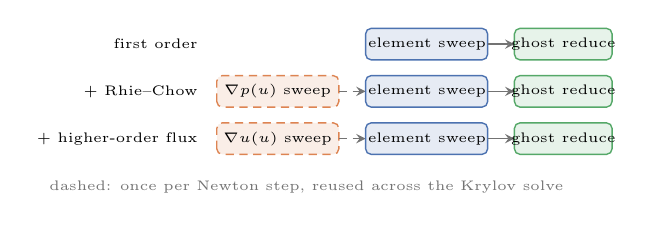
\begin{tikzpicture}[scale=1.00,font=\scriptsize]
  \node[anchor=east,font=\tiny] at (2.23,1.40) {first order};
  \draw[PackA,fill=PackA!14,rounded corners=2pt,line width=0.5pt] (4.24,1.20) rectangle (5.79,1.60);
  \node[font=\tiny,align=center] at (5.02,1.40) {element sweep};
  \draw[->,>=stealth,black!55,line width=0.5pt] (5.79,1.40) -- (6.13,1.40);
  \draw[PackC,fill=PackC!14,rounded corners=2pt,line width=0.5pt] (6.13,1.20) rectangle (7.37,1.60);
  \node[font=\tiny,align=center] at (6.75,1.40) {ghost reduce};
  \node[anchor=east,font=\tiny] at (2.23,0.80) {$+$ Rhie--Chow};
  \draw[PackB,fill=PackB!14,rounded corners=2pt,line width=0.5pt,densely dashed] (2.35,0.60) rectangle (3.90,1.00);
  \node[font=\tiny,align=center] at (3.12,0.80) {$\nabla p(u)$ sweep};
  \draw[->,>=stealth,black!55,line width=0.5pt,densely dashed] (3.90,0.80) -- (4.24,0.80);
  \draw[PackA,fill=PackA!14,rounded corners=2pt,line width=0.5pt] (4.24,0.60) rectangle (5.79,1.00);
  \node[font=\tiny,align=center] at (5.02,0.80) {element sweep};
  \draw[->,>=stealth,black!55,line width=0.5pt] (5.79,0.80) -- (6.13,0.80);
  \draw[PackC,fill=PackC!14,rounded corners=2pt,line width=0.5pt] (6.13,0.60) rectangle (7.37,1.00);
  \node[font=\tiny,align=center] at (6.75,0.80) {ghost reduce};
  \node[anchor=east,font=\tiny] at (2.23,0.20) {$+$ higher-order flux};
  \draw[PackB,fill=PackB!14,rounded corners=2pt,line width=0.5pt,densely dashed] (2.35,0.00) rectangle (3.90,0.40);
  \node[font=\tiny,align=center] at (3.12,0.20) {$\nabla u(u)$ sweep};
  \draw[->,>=stealth,black!55,line width=0.5pt,densely dashed] (3.90,0.20) -- (4.24,0.20);
  \draw[PackA,fill=PackA!14,rounded corners=2pt,line width=0.5pt] (4.24,0.00) rectangle (5.79,0.40);
  \node[font=\tiny,align=center] at (5.02,0.20) {element sweep};
  \draw[->,>=stealth,black!55,line width=0.5pt] (5.79,0.20) -- (6.13,0.20);
  \draw[PackC,fill=PackC!14,rounded corners=2pt,line width=0.5pt] (6.13,0.00) rectangle (7.37,0.40);
  \node[font=\tiny,align=center] at (6.75,0.20) {ghost reduce};
  \node[anchor=west,font=\tiny,black!55] at (0.10,-0.42) {dashed: once per Newton step, reused across the Krylov solve};
\end{tikzpicture}
